\documentclass[12pt,a4paper]{memoir}

% substituir linha seguinte por 
% \usepackage[english]{babel} 
% se o relatório for escrito na língua inglesa.
\usepackage[portuguese]{babel}

% \usepackage[utf8]{inputenc}
\usepackage[T1]{fontenc}

\usepackage{makeidx}
\usepackage{xspace}
\usepackage{graphicx,color,times}
\usepackage{fancyhdr}
% \usepackage{pxfonts}
% \usepackage{times}
% \usepackage{mathptm}
% \usepackage{amssymb}
% \usepackage{amsfonts}

\usepackage{minted}
\usepackage{paralist}
\usepackage{enumitem}
\usepackage{booktabs}
\usepackage{amssymb}
\usepackage{calc}
\usepackage{array}
%\usepackage{color}
%\usepackage{colortbl}
\usepackage{xcolor}

\usepackage{caption}
\usepackage{subcaption}

\usepackage{amsmath}
\usepackage{latexsym}
\usepackage[printonlyused]{acronym}
\usepackage{float}
\usepackage{listings}
\usepackage{tocbibind}
% \usepackage{natbib}
\usepackage{hyperref}

% \usepackage{glossaries}
% \makeglossaries

% \renewcommand{\ttdefault}{phv}

\pagestyle{fancy}
\renewcommand{\chaptermark}[1]{\markboth{#1}{}}
\renewcommand{\sectionmark}[1]{\markright{\thesection\ #1}}
\fancyhf{} \fancyhead[LE,RO]{\bfseries\thepage}
\fancyhead[LO]{\bfseries\rightmark}
\fancyhead[RE]{\bfseries\leftmark}
\renewcommand{\headrulewidth}{0.5pt}
\renewcommand{\footrulewidth}{0pt}
\setlength{\headheight}{15.6pt}
\setlength{\marginparsep}{0cm}
\setlength{\marginparwidth}{0cm}
\setlength{\marginparpush}{0cm}
\addtolength{\hoffset}{-1.0cm}
\addtolength{\oddsidemargin}{\evensidemargin}
\addtolength{\oddsidemargin}{0.5cm}
\addtolength{\evensidemargin}{-0.5cm}


\usepackage{fix-cm}
\usepackage{fourier}
\usepackage[scaled=.92]{helvet}
\definecolor{ChapGrey}{rgb}{0.6,0.6,0.6}
\newcommand{\LargeFont}{
	\usefont{\encodingdefault}{\rmdefault}{b}{n}
	\fontsize{60}{80}\selectfont\color{ChapGrey}
}
\makeatletter
\makechapterstyle{GreyNum}{
	\renewcommand{\chapnamefont}{\large\sffamily\bfseries\itshape}
	\renewcommand{\chapnumfont}{\LargeFont}
	\renewcommand{\chaptitlefont}{\Huge\sffamily\bfseries\itshape}
	\setlength{\beforechapskip}{0pt}
	\setlength{\midchapskip}{40pt}
	\setlength{\afterchapskip}{60pt}
	\renewcommand\chapterheadstart{\vspace*{\beforechapskip}}
	\renewcommand\printchaptername{
		\begin{tabular}{@{}c@{}}
			\chapnamefont \@chapapp\\}
		\renewcommand\chapternamenum{\noalign{\vskip 2ex}}
		\renewcommand\printchapternum{\chapnumfont\thechapter\par}
		\renewcommand\afterchapternum{
		\end{tabular}
		\par\nobreak\vskip\midchapskip}
	\renewcommand\printchapternonum{}
	\renewcommand\printchaptertitle[1]{
		{\chaptitlefont{##1}\par}}
	\renewcommand\afterchaptertitle{\par\nobreak\vskip \afterchapskip}
}
\makeatother
\chapterstyle{GreyNum}

\setcounter{tocdepth}{3}
\setsecnumdepth{subsubsection}

\renewcommand{\ttdefault}{lmtt}


% NEW COLORS
\definecolor{dark}{gray}{0.25}
\definecolor{lgray}{gray}{0.9}
\definecolor{dkblue}{rgb}{0,0.13,0.4}
\definecolor{dkgreen}{rgb}{0,0.6,0}
\definecolor{gray}{rgb}{0.5,0.5,0.5}
\definecolor{mauve}{rgb}{0.58,0,0.82}

\lstset{ %
	language=C,                    basicstyle=\footnotesize,
	numbers=none,                  numberstyle=\tiny\color{gray}, 
	stepnumber=1,                  numbersep=5pt,
	backgroundcolor=\color{white}, showspaces=false,
	showstringspaces=false,        showtabs=false,
	frame=single,                  rulecolor=\color{black},
	tabsize=2,                     captionpos=b,
	breaklines=true,               breakatwhitespace=false,
	title=\lstname,                keywordstyle=\color{blue},
	commentstyle=\color{dkgreen},  stringstyle=\color{mauve},
	escapeinside={\%*}{*)},        morekeywords={*},
	belowskip=0cm
}

% \renewcommand{\lstlistingname}{Excerto de Código}
% \renewcommand{\lstlistlistingname}{Lista de Excertos de Código}

% \renewcommand{\today}{\day \ifcase \month \or janeiro\or fevereiro\or março\or %
	% abril\or maio\or junho\or julho\or agosto\or setembro\or outubro\or novembro\or %
	% dezembro\fi de \number \year}

\newcommand{\famousquote}[2]{
	\begin{quote}
		\rule{\textwidth-2\leftmargin}{0.4pt}
		{\itshape #1}
		\vspace{-12pt}
		\begin{flushright}
			\textasciitilde~#2
		\end{flushright}
		\vspace{-20pt}
		\rule{\textwidth-2\leftmargin}{0.4pt}
	\end{quote}
}

\graphicspath{{./img/}}
\newcommand{\usecasescale}{0.5}

\newcommand{\registered}{\textsuperscript{\textregistered}}
\newcommand{\ccopyright}{\textsuperscript{\textcopyright}}

\newcommand{\theteam}{Diogo Simões}
\newcommand{\theapp}{\emph{CalcGL}}
\newcommand{\theappdescription}{Visualização de funções implícitas por \emph{ray marching}}
\newcommand{\groupname}{{\itshape\theteam}}
\newcommand{\appname}{\emph{\theapp}:~{\emph{\theappdescription}}}
\newcommand{\opengl}{\textit{OpenGL}\registered}

\newcommand{\revision}[1]{{\color{orange}[!Rev] #1}}
\newcommand{\todo}[1]{{\color{red}[!TODO] #1}}
\newcommand{\hint}[1]{{\color{green!50!black}[!Hint] #1}}


\begin{document}
	\thispagestyle{empty}
\setcounter{page}{-1}

\begin{center}
\begin{Huge}
\textbf{Universidade da Beira Interior}
\end{Huge}
\end{center}

\begin{center}
\begin{Huge}
Departamento de Informática
\end{Huge}
\end{center}

\vspace{0,07cm}
\begin{figure}[!htb]
\centering

\includegraphics[width=191pt]{ubi-fe-di.png}
\end{figure}

\vspace{0.5cm}
\begin{center}
\begin{Large}
\textbf{N\textordmasculine{} 121 --- 2022}\\
\textbf{\emph{\theappdescription}}
\end{Large}
\end{center}


\vspace{0.5cm}
\begin{center}
\begin{normalsize}
\begin{large}
Elaborado por:
\end{large}
\end{normalsize}
\end{center}

\vspace{0.2cm}
\begin{center}
\begin{large}
\textbf{Diogo Castanheira Simões}
\end{large}
\end{center}

\vspace{0,5cm}
\begin{center}
\begin{normalsize}
\begin{large}
Orientador:
\end{large}
\end{normalsize}
\end{center}

\vspace{0.2cm}
\begin{center}
\begin{large}
\textbf{Professor Doutor Abel João Padrão Gomes}
\end{large}
\end{center}



\vspace{0.5cm}
\begin{center}
\begin{normalsize}
\today
\end{normalsize}
\end{center}

	
	\clearpage{\thispagestyle{empty}\cleardoublepage}
	\frontmatter
	\chapter*{Agradecimentos}
\label{ch::ack}

\todo{}

Agradeço ao meu professor orientador, Prof. Doutor Abel João Padrão Gomes.

	
	\clearpage{\thispagestyle{empty}\cleardoublepage}
	\tableofcontents
	
	\clearpage{\thispagestyle{empty}\cleardoublepage}
	\listoffigures
	
	% #   ATENÇÃO
	% Se não existirem tabelas, comentar as duas linhas seguintes
	\clearpage{\thispagestyle{empty}\cleardoublepage}
	\listoftables
	
	% #   ATENÇÃO
	% Se existirem trechos de código, descomentar as seguintes linhas
	% \clearpage{\thispagestyle{empty}\cleardoublepage}
	% \lstlistoflistings
	
	\clearpage{\thispagestyle{empty}\cleardoublepage}
	\chapter*{Acrónimos}
\label{ch::acro}

% #   ATENÇÃO
% A lista de acrónimods deve ser ordenada alfanumericamente.
% Estrangeirismos devem ser realçados em itálico.
% Se o relatório for escrito em Inglês, uma palavra portuguesa é um estrangeirismo.

% O maior acrónimo deve ser colocado neste ponto (reparar que CFIUTE é maior que TCP!).
%               vvvvvv
\begin{acronym}[SIGGRAPH]
    \acro{API}{\emph{Application Programming Interface}}
    \acro{ASCII}{\emph{American Standard Code for Information Interchange}}
    \acro{CBO}{\emph{Color Buffer Object}}
    \acro{CG}{Computação Gráfica}
    \acro{CPU}{\emph{Central Processing Unit}}
    \acro{CUDA}{\emph{Compute Unified Device Architecture}}
    \acro{FOV}{\emph{Field of View}}
    \acro{GLAD}{\emph{Multi-Language GL/GLES/EGL/GLX/WGL Loader-Generator}}
    \acro{GLEW}{\emph{OpenGL Extension Wrangler Library}}
    \acro{GLM}{\emph{OpenGL Mathematics}}
    \acro{GLSL}{\emph{OpenGL Shader Language}}
    \acro{GPU}{\emph{Graphics Processing Unit}}
    \acro{GUI}{\emph{Graphical User Interface}}
    \acro{MVP}{\emph{Model-View-Projection}}
    \acro{RAM}{\emph{Random Access Memory}}
    \acro{RM}{Ressonância Magnética}
    \acro{SDF}{\emph{Signed Distance Function}}
    \acro{SGI}{\emph{Silicon Graphics}}
    \acro{SIGGRAPH}{\emph{Special Interest Group on Computer Graphics and Interactive Techniques}}
    \acro{SISM}{\emph{Smart Interactive State Machine}}
    \acro{SoC}{\emph{System on a Chip}}
    \acro{SSBO}{\emph{Shader Storage Buffer Object}}
    \acro{SWOT}{\emph{Strength, Weakness, Opportunity, and Threat Analysis}}
    \acro{TI}{Tecnologias de Informação}
    \acro{UBI}{Universidade da Beira Interior}
    \acro{UC}{Unidade Curricular}
    \acro{URI}{\emph{Uniform Resource Identifier}}
    \acro{VAO}{\emph{Vertex Attribute Object}}
    \acro{VBO}{\emph{Vertex Buffer Object}}
    \acro{VRAM}{\emph{Video Random-Access Memory}}
    \acro{WSL}{\emph{Windows Subsystem for Linux}}
    \acro{WSLg}{\acl{WSL} \emph{\acs{GUI}}}
\end{acronym}

	
	% \clearpage{\pagestyle{empty}\cleardoublepage}
	% \chapter*{Glossário}
\makeglossaries

\newglossaryentry{.NET Framework}
{
  name={.NET Framework},
  description={É uma plataforma para desenvolvimento e funcionamento de aplicações desenvolvida pela Microsoft.}
}

\newglossaryentry{ASP.NET}
{
  name={ASP .Net},
  description={É uma plataforma da Microsoft para o desenvolvimento de aplicações Web e é o sucessor da tecnologia ASP.}
}

\newglossaryentry{CS}
{
  name={C\#},
  description={Lê-se \textit{C Sharp} e é uma linguagem de programação orientada a objectos, desenvolvida pela Microsoft, inicialmente para a plataforma .NET. O C\# é inspirado na junção entre as linguagens C++ e Java.}
}


\newglossaryentry{Java}
{
  name={JAVA},
  description={É uma linguagem de programação orientada a objectos, desenvolvida pela Sun Microsystems na década de 90. Hoje pertence à empresa Oracle.}
}


\newglossaryentry{OpenDMTP}
{
  name={OpenDMTP},
  description={\textit{Open Device Monitoring and Tracking Protocol} é um protocolo e uma \textit{framework} abertos que permite a comunicação bidireccional entre servidores e clientes através da internet.}
}


\newglossaryentry{OpenGTS}
{
  name={Open GTS},
  description={É o primeiro projecto \textit{Open Source} \textit{Web-Based} para controlo de frotas por GPS.}
}


\newglossaryentry{VS2010}
{
  name={Visual Studio 2010},
  description={\textit{Microsoft Visual Studio 2010} é um sistema de desenvolvimento desenvolvido pela Microsoft e é dedicado ao Framework .NET, que contem um conjunto de ferramentas de desenvolvimento projectadas para auxiliar os programadores a enfrentarem desafios complexos.}
}


\newglossaryentry{WebS}
{
	name={Web Service},
	description={Web services são aplicações modulares auto-descritas e auto-contidas, que permitem a integração de sistemas e a comunicação entre aplicações de diferentes tipos.}
}


\newglossaryentry{WebBased}
{
	name={Web Based},
	description={Aplicação desenvolvida para a Web.}
}

\newglossaryentry{Roaming}
{
	name={Roaming},
	description={Define a possibilidade de um utilizador de uma determinada rede obter rede/conecção fora da área geográfica onde foi registado.}
}


\newglossaryentry{Smartphone}
{
	name={Smartphone},
	description={Smartphone é um telefone móvel que contem muitas das principais tecnologias de comunicação e serviços que existem nos computadores pessoais, como acesso a e-mails, serviços de mensagens instantâneas, internet, GPS, entre outros.}
}

\newglossaryentry{TCPIP}
{
	name={TCP/IP},
	description={É um conjunto de protocolos de comunicação entre computadores ligados rede. O nome TCP/IP surge da união entre dois protocolos: o TCP (Transmission Control Protocol) e o protocolo IP (Internet Protocol).}
}

\newglossaryentry{Firewall}
{
	name={Firewall},
	description={É o nome criado para definir um dispositivo para uma rede de computadores que tem como objectivo criar uma política de segurança num determinado ponto de controlo da rede.}
}

\newglossaryentry{JavaScript}
{
	name={JavaScript},
	description={É uma linguagem de programação baseada na linguagem de programação ECMAScript. Actualmente é a linguagem de programação mais utilizada em \textit{``Client-Side''} nos \textit{browsers}.}
}

\newglossaryentry{Flash}
{
	name={Flash},
	description={Desenvolvido pela Macromedia, o Flash é um software utilizado para criação de animações interactivas que funcionam incorporadas em \textit{Browsers}, \textit{Desktop}, \textit{Smartphones}, \textit{Tablets}, e Televisores.}
}


\newglossaryentry{StoredProcedure}
{
	name={Stored Procedure },
	description={É o nome dado a um conjunto de comandos numa base de dados de forma a simplificar a sua utilização.}
}

\newglossaryentry{SQLS}
{
	name={SQL Server 2008},
	description={É um sistema de gestão de base de dados relacional criado pela Microsoft.}
}

\newglossaryentry{Firm}
{
	name={Firmware},
	description={É o conjunto de instruções operacionais programadas directamente no \textit{hardware} de um equipamento electrónico.}
}

\newglossaryentry{browser}
{
	name={Browser},
	description={É um programa de computador que possibilita aos utilizadores uma interacção com documentos virtuais da Internet, também conhecidos como páginas Web.}
}


	
	\clearpage{\thispagestyle{empty}\cleardoublepage}
	
	\mainmatter
	\acresetall
	\chapter{Introdução}
\label{ch::intro}

\section{Enquadramento}
\label{sec::intro:enquadramento}

%O estudo matemático de funções levou à descoberta de diferentes métodos para a sua representação e análise, nomeadamente os modelos explícitos, paramétricos e implícitos. Contudo, apenas as funções explícitas são trivialmente renderizadas por computadores; estas representam grandes desafios uma vez que nem sempre é possível obter expressões explícitas.
%
%Neste sentido, o estudo de funções implícitas torna-se vital para inúmeros fins, pelo que a sua renderização computacional tem sido alvo de estudo por décadas. Os resultados dos enormes avanços feitos na área são atualmente desfrutados por milhões de pessoas, tanto a título pessoal como no mundo empresarial e de investigação.


O processo de síntese de imagem em computação gráfica é na sua essência a transformação de geometria em pixéis. 
As duas técnicas mais usuais de o fazer são: renderização e \emph{ray casting}. Na renderização, a geometria é dada por uma malha de triângulos
e é o próprio sistema gráfico (e.g., OpenGL ou DirectX) que transforma os triângulos em pixéis. 
No \emph{ray casting}, o processo é diferente pois emitem-se raios (um por pixel) a partir da câmara (i.e., o olho do observador) numa cena, calculando-se então os pontos de intersecção entre os raios e a geometria de cada objeto existente na cena. 
No caso presente, utilizou-se o \emph{ray marching}, que é uma variante do \emph{ray casting}.

Obviamente, a geometria de cada objeto tem uma dada representação matemática. As representações matemáticas da geometria destes objetos são dadas por funções analíticas. As representações são de três tipos: explícitas, paramétricas e implícitas. No trabalho descrito neste relatório, utilizaram-se funções implícitas para descrever a geometria de cada objeto.


\section{Motivação}
\label{sec::intro:motivacao}

As versões modernas do \opengl~(i.e. a partir da versão 3.3) permitem que o programador escreva os seus próprios \textit{shaders} a serem utilizados na \textit{pipeline} de renderização. Uma consequência imediata é a possibilidade de paralelizar inúmeros cálculos que normalmente seriam realizados pela \ac{CPU}.

Ainda assim, uma miríade de \textit{software} de renderização não tira proveito de tais capacidades. Desta forma, é de interesse estudar um algoritmo de renderização por volume e analisar a sua potencial paralelização.


\section{Objetivos}
\label{sec::intro:objetivos}

O presente projeto tem por \textbf{objetivo principal} implementar um sistema de visualização de funções implícitas.

Este tem ainda os seguintes \textbf{objetivos secundários}:
\begin{itemize}
	\item Estudar funções implícitas e o cálculo das respetivas iso-superfícies;
	\item Analisar o modelo de renderização por volume;
	\item Implementar o algoritmo de \textit{ray marching} em particular;
	\item Implementar aceleração por \textit{hardware} através da programação de \emph{shaders} em \opengl.
    \item Avaliar as diferenças entre \ac{CPU} \textit{single-threaded}, \ac{CPU} \textit{multi-threaded} e acelerado por \ac{GPU}.
\end{itemize}


\section{Organização do Documento}
\label{sec::intro:orgdoc}

O presente relatório estrutura-se em seis capítulos:

\begin{enumerate}
	\item No primeiro capítulo --- \textbf{Introdução} --- é apresentado o projeto, em particular o seu enquadramento e motivação, assim como os seus objetivos e a respetiva organização do relatório.
	
	\item No segundo capítulo --- \textbf{Estado da Arte} --- são apresentados os conceitos fundamentais de funções implícitas, assim como métodos usados para renderizar, com particular foco no algoritmo \textit{Ray Marching}. É também feita uma introdução aos conceitos introdutórios do \opengl~moderno.
	
	\item No terceiro capítulo --- \textbf{Tecnologias e Ferramentas} --- são definidos os conjuntos de tecnologias, ferramentas e \textit{hardware} usados para a implementação do projeto.
	
	\item No quarto capítulo --- \textbf{Implementação} --- são descritas as decisões e detalhes tomados durante o desenvolvimento, em conjunto com o funcionamento do programa e os seus requisitos.
	
	\item No quinto capítulo --- \textbf{Testes e Resultados} --- é demonstrado o funcionamento do programa final, os resultados por si obtidos e as diferentes fases de teste.
	
	\item No sexto capítulo --- \textbf{Conclusões e Trabalho Futuro} --- é feita a reflexão sobre os conhecimentos obtidos ao longo do desenvolvimento do projeto, os seus obstáculos, o que não foi possível alcançar e o que poderá ser explorado no futuro.
\end{enumerate}

	\clearpage{\thispagestyle{empty}\cleardoublepage}
	% !TeX spellcheck = pt_BR
\chapter{Estado da Arte}
\label{ch::arte}

\section{Introdução}
\label{sec::arte:intro}

A visualização computacional de funções é a base de muitas aplicações práticas em computação gráfica, tais como em videojogos e visualização molecular. O estudo destas funções permite igualmente outro tipo de cálculos, tais como colisões.

Para alcançar os objetivos propostos no presente projeto, é imperativo estudar os seguintes tópicos:

\begin{itemize}
	\item Funções implícitas;
	\item Técnicas de renderização em geral e algoritmos volumétricos em particular;
	\item Uso da \ac{API} \opengl e programação em \ac{GLSL}.
\end{itemize}


\section{Funções Implícitas}
\label{sec::arte:implicitas}

%\subsection{Definição e Aplicações}
%\label{ssec::arte:implicitas:def}

% O que é? Exemplo(s). Que aplicações têm?

Às funções definidas em função de uma variável dá-se o nome de \textbf{funções explícitas}. Exemplos clássicos em $\mathbb{R}^2$ incluem equações de retas ($y = mx + b$) e parábolas ($y = ax^2 + bx + c$). Ora, nem todos os subconjuntos de pontos no espaço cartesiano podem ser definidos por funções explícitas. Um exemplo comum em $\mathbb{R}^2$ é a circunferência (Figura \ref{fig::circumference}):

\begin{equation}
	(x - x_0)^2 + (y - y_0)^2 = r^2
	\label{eq::circ_implicita}
\end{equation}

onde $(x_0, y_0)$ é o centro e $r$ o raio.

\begin{figure}[!htbp]
	\centering
	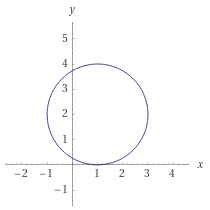
\includegraphics[scale=1.0]{circumference}
	\caption[Exemplo de uma circunferência]{Exemplo de uma circunferência de centro $(1, 2)$ e raio $2$.}
	\label{fig::circumference}
\end{figure}

Sendo uma equação de segundo grau, é possível representá-la através de duas funções explícitas:

\begin{eqnarray}
		y = y_0 + \sqrt{r^2 - (x - x_0)^2} \\
		y = y_0 - \sqrt{r^2 - (x - x_0)^2}
\end{eqnarray}

Esta transformação não é possível para todos os polinómios, em particular para graus superiores a $4$. Contudo, estas expressões polinomiais continuam a ser subconjuntos válidos de $\mathbb{R}^n$, necessitando então de formas alternativas de representação. Dois métodos e respetivas representações da circunferência são:

\begin{enumerate}
	\item \textbf{Funções paramétricas}: cada eixo é definido em ordem a uma variável adicional $t$:
	\begin{equation}
		\left\{\begin{array}{l}
			x = r\cos(t) \\
			y = r\sin(t)
		\end{array}\right.
	\label{eq::circ_parametrica}
	\end{equation}
	
	\item \textbf{Funções implícitas}: a equação não é definida a ordem a uma variável em particular (equação (\ref{eq::circ_implicita})).
\end{enumerate}

Uma \textbf{função implícita} é então definida por $f~:~\mathbb{R}^n \longrightarrow \mathbb{R}$, ou seja, para qualquer ponto em $\mathbb{R}^n$ é determinado um resultado em $\mathbb{R}$. Dependendo da função, o valor obtido pode ter significado, tal como uma grandeza física (\textit{e.g.} densidade de um líquido ou sua temperatura a cada ponto do espaço). Esta função diz-se \textbf{algébrica} caso seja polinomial em cada variável.

Por seu turno, em $\mathbb{R}^3$, a \textbf{iso-superfície} de uma função implícita é a superfície que satisfaz a condição $f(\mathbf{x}) = 0$ (onde, doravante, $\mathbf{x} \equiv (x,y,z)$). Esta pode ser suavizada através de um parâmetro $s \in \mathbb{R}$ tal que $f(\mathbf{x}) - s = 0$. Este efeito é utilizado diretamente e com sucesso nas Superfícies $\Pi$ \cite{Raposo2019}.


\todo{Mais aplicações.}


%\subsection{Desafios Computacionais}
%\label{ssec::arte:implicitas:desafios}


\section{Técnicas de Renderização: Visão Geral}
\label{sec::arte:render}

Muitos algoritmos de renderização têm vindo a ser investigados e usado em \textit{software} que implemente diversas técnicas para obter uma imagem final.\\


A nossa visão capta a luz refletida por objetos num determinado cenário. Durante o processo, a maioria dos comprimentos de onda das fontes de luz são absorvidos sendo o restante refletido. Como resultado final, os comprimentos de onda refletidos e captados pelos olhos constituem o que é interpretado como cor.

No entanto, o cálculo do percurso para cada partícula de luz num determinado cenário é na grande maioria dos casos algo impraticável devido à grande demora da obtenção dos resultados.

Por dito motivo, foram desenvolvidos métodos mais eficientes de cálculo da luz:
\begin{itemize}
    \item \textbf{Rasterização}, técnica ainda usada na pipeline do \opengl. Consiste na conversão numa imagem descrita geometricamente numa série de pixeis que quando juntos criam a imagem.
    
    \item \textbf{Ray Casting}, considera um cenário a ser observado por um determinado ponto de vista, o mesmo calcula a imagem observada baseado apenas na geometria e em leis óticas básicas.
    
    \item \textbf{Ray Tracing}, bastante próximo a como Ray Casting funciona, no entanto implementa também simulações ótica mais avançadas.
\end{itemize}

\hint{Breve introdução às categorias de técnicas/algoritmos de renderização.}\\
\revision{Categorização das técnicas.}


As funções implícitas representam simultaneamente uma grande oportunidade na área da computação gráfica e um enorme desafio. Se por um lado é possível obter a visualização de formas geométricas complexas com recurso a funções implícitas, por outro não há um método direto de determinar quais os pontos da iso-superfície.

Vários algoritmos têm sido propostos ao longo das últimas décadas, tais como \textit{marching cubes}\cite{Lorensen1987}, \textit{ray marching}, \textit{sphere tracing}\cite{Hart1996} e \textit{ray tracing}.

\begin{itemize}
	%\item \textbf{Rasterização}:\\
	%\hint{Técnica ainda utilizada na pipeline do OpenGL na fase final.}
	
	\item \textbf{Triangulação}:\\
	A iso-superfície é dividida em triângulos, os quais formam a \textit{mesh} a ser renderizada pela \ac{GPU}. Um exemplo é o algoritmo de \textit{Marching Cubes}\cite{Lorensen1987} no qual o espaço é dividido em cubos onde o valor da função implícita é calculado para cada vértice. A análise dos sinais permite determinar quais arestas do cubo a superfície interseta, num total de 256 possíveis combinações de triângulos.
	
	\item \textbf{\textit{Ray Tracing} e algoritmos volumétricos}:\\
    
	
	\item \hint{Mais técnicas/algoritmos?}
\end{itemize}


\section{\emph{Ray Marching}}
\label{sec::arte:raymarch}

\hint{Como funciona o algoritmo? É paralelizável? Se sim, como e porquê?}

\textit{Ray marching} é uma simples técnica que tal como no tradicional \textit{ray tracing}, não é tão simples de resolver uma superfície (ou até impossível caso sem o uso de métodos numéricos interativos). Em \textit{ray tracing} apenas nos focamos na interseção do raio emitido com a superfície, enquanto no algoritmo de \textit{ray marching} marchamos na direção tomada até encontrarmos uma interseção (isto se a mesma existir).\\

Isto é nos interessante caso:
\begin{itemize}
    \item precisemos de renderizar volumes que não são uniformes;
    \item renderizemos funções implícitas ou fractais;
    \item tenhamos interesse em renderizar outros tipos de funções paramétricas onde a interseção não é conhecida antecipadamente, como \textit{parallel mapping};
\end{itemize}

\subsection{Sphere Tracing}
\textit{Sphere tracing} é um possível algoritmo de \textit{ray marching}. No entanto, nem todos os usos de \textit{ray marching} beneficiam deste método, porque estes não conseguem ser convertidos para este esquema.

\textit{Sphere tracing} é usado para renderizar \textbf{superfícies implícitas}.
Porque esta função pode ser resolvida a cada ponto, podemos ir em frente e estimar a maior esfera possível que possa caber no atual passo de marcha. Então sabemos que a próxima distancia a marchar é pelo menos tão grande quanto o raio da dita esfera. Desta forma adaptamos então o numero de passos a marchar e tornamos com o processo muito mais rápido.

\todo{Adicionar imagem de exemplo algoritmo naive em 2D}\\




O algoritmo geral de \textit{ray marching} contempla os seguintes quatro passos:

\begin{enumerate}
	\item \textbf{\textit{Ray casting}}:
	
	\item \textbf{\textit{Sampling}}:
	
	\item \textbf{\textit{Shading}}:
	
	\item \textbf{\textit{Compositing}}:
\end{enumerate}


\section{\opengl}
\label{sec::arte:opengl}

\hint{Não recomendo um rip-off do meu relatório, mas ele pode servir de base para esta secção, tentando melhorá-lo e corrigir possíveis gafes.}


\section{Conclusões}
\label{sec::arte:conc}

\ldots Whiskas Saquetas.

	\clearpage{\thispagestyle{empty}\cleardoublepage}
	\chapter{Tecnologias e Ferramentas}
\label{ch::tecno}

\section{Introdução}
\label{sec::tecno:intro}

Bla bla inicial\ldots


\section{Tecnologias}
\label{sec::tecno:tecno}

Para a implementação do projeto \theapp~com \opengl~foi escolhida a linguagem de programação C++. A fim de melhorar a experiência de utilização do \opengl, foram utilizadas as seguintes bibliotecas e \textit{frameworks}:

\begin{itemize}
    %\item \textbf{C++}: Linguagem compilada de uso geral multi-paradigma. Desenvolvida por Bjarne Stroustrup.
    
    \item \textbf{GLFW~\cite{glfw}}: \ac{API} simplificada para o \opengl, igualmente multi-plataforma, permitindo a gestão de janelas, contextos, superfícies e comandos (rato, teclado e \textit{joystick});
    
    \item \textbf{\acs{GLAD}~\cite{glad,glad-webservice}} (\acl{GLAD}): gerador automático de \textit{loaders} para \opengl;
    
    \item \textbf{\acs{GLM}~\cite{glm}} (\acl{GLM}): biblioteca matemática baseada na linguagem dos \textit{shaders} do \opengl, \ac{GLSL}.
    
    \item \textbf{\textit{FreeType}~\cite{freetype}}: biblioteca de desenvolvimento dedicada à renderização de fontes em \textit{bitmaps} utilizáveis, por exemplo, pelo \opengl.
    
    % \item \textbf{\acs{GLSL}} (\acl{GLSL}): principal linguagem de \textit{shading} para \opengl.
    
    % \item \textbf{\opengl~\cite{opengl}}: \ac{API} multi-plataforma e com suporte a múltiplas linguagens de programação para a renderização de gráficos vetoriais 2D e 3D com recurso à placa gráfica;
\end{itemize}

Há ainda a notar que a \ac{GPU} é programada através de \textit{shaders} com a linguagem \acf{GLSL}.

As versões destas bibliotecas e outro \textit{software} auxiliar utilizado estão sumariados na Tabela \ref{tab::ferramentas}.

\begin{table}[!p]
    \centering
    \caption[Ferramentas utilizadas]{Ferramentas e tecnologias utilizadas, organizadas por categoria.}
    \label{tab::ferramentas}
    \begin{tabular}{p{1cm} l l}
        \toprule
        & {\bfseries \textit{Software} / Tecnologia} & {\bfseries Versão} \\
        \midrule
        \multicolumn{3}{l}{\bfseries Aplicação \opengl} \\
        & \opengl           & 4.6 \\
        & GLFW              & 3.3.5 \\
        & \acs{GLAD}        & 0.1.34 \\
        & \acs{GLM}         & 0.9.9.8 \\
        & \textit{FreeType} & 2.10.4 \\
        \midrule
        \multicolumn{3}{l}{\bfseries Relatório} \\
        & Xe\TeX & 3.141592653-2.6-0.999993 \\
        &\textit{TeXstudio}\ccopyright & 4.2.2 \\
        \midrule
        \multicolumn{3}{l}{\bfseries Controlo de versões} \\
        & \textit{git} & 2.36.1 \\
        & \textit{GitKraken} & 8.6.1  \\
        \bottomrule
    \end{tabular}
\end{table}



\section{Código \emph{Open Source}}
\label{sec::tecno:opensource}

Além das bibliotecas e \textit{frameworks} referidas na Secção \ref{sec::tecno:tecno}, código \textit{open source} adicional foi utilizado para facilitar a implementação de componentes que não fazem parte do objetivo de estudo do projeto. Estes são:

\begin{itemize}
    \item \textbf{\textit{CParser}} \todo{Citação}: biblioteca para \textit{parsing} de uma sequência de caracteres como uma expressão usando o algoritmo \textit{Shunting-yard} de Dijkstra;
    
    \item \todo{Código do Learn OpenGL}
    
    \item \hint{quickGL??}
\end{itemize}


\section{\textit{Hardware}}
\label{sec::tecno:hw}

O \textit{software} final foi testado em três computadores distintos, listados na Tabela \ref{tab::hardware}.

\begin{table}[!p]
	\centering
	\caption[Lista de \textit{hardware} para testes]{Lista de \textit{hardware} onde o projeto \theapp~foi testado.}
	\label{tab::hardware}
	\begin{tabular}{p{1cm} l l}
		\toprule
		%& {\bfseries Componente} & {\bfseries } \\
		%\midrule
		\multicolumn{3}{l}{\bfseries Computador portátil 1} \\
		& Processador (\acs{CPU})   & Intel\registered~i5-8300H (2.3--4.0GHz) \\
		& Placa gráfica (\acs{GPU}) & NVidia\registered~GTX 1050 Ti (4GB) \\
		& Memória \acs{RAM}         & 16GB (DDR4 2133MHz) \\
		& Armazenamento             & 256GB (PCIe 3.0 x4) \\
		\midrule
		\multicolumn{3}{l}{\bfseries Computador portátil 2} \\
		& Processador (\acs{CPU})   & AMD Ryzen\texttrademark~9 5900HS (3.0--4.6GHz) \\
		& Placa gráfica (\acs{GPU}) & NVidia\registered~RTX 3050 Ti (4GB) \\
		& Memória \acs{RAM}         & 16GB (DDR4 3200MHz) \\
		& Armazenamento             & SSD NVMe 1TB (PCIe 3.0 x4) \\
		\midrule
		\multicolumn{3}{l}{\bfseries Computador \textit{desktop}} \\
		& Processador (\acs{CPU})   & AMD Ryzen\texttrademark~7 2700X (3.7--4.3GHz) \\
		& Placa gráfica (\acs{GPU}) & NVidia\registered~RTX 3070 (8GB) \\
		& Memória \acs{RAM}         & 32GB (DDR4 3200MHz) \\
		& Armazenamento             & SSD NVMe 1TB (PCIe 3.0 x4) \\
		\bottomrule
	\end{tabular}
\end{table}


\section{Conclusões}
\label{sec::tecno:conc}

\ldots Whiskas Saquetas.

	\clearpage{\thispagestyle{empty}\cleardoublepage}
	\chapter{Implementação}
\label{ch::impl}

%\section{Introdução}
%\label{sec::impl:intro}

A implementação do projeto \theapp~será detalhada no presente Capítulo, com particular foco nos seguintes pontos:

\begin{itemize}[nosep]
	\item Requisitos funcionais do projeto;
	\item Estrutura do código e o fluxo do mesmo;
	\item Detalhes de implementação e desafios encontrados.
\end{itemize}


\section{Funcionalidades e Requisitos}
\label{sec::impl:requisitos}

O projeto \theapp~segue uma lista de \textbf{funcionalidades} a implementar baseados nos objetivos do projeto (Secção \ref{sec::intro:objetivos}), em específico:

\begin{itemize}
    \item Renderização de funções implícitas com uso de \textit{ray marching};
    \item Suporte a dois motores de cálculo:
    \begin{enumerate}[nosep]
        \item Por \textit{software} (i.e. os cálculos são efetuados pela \ac{CPU});
        \item Aceleração por \textit{hardware} (com uso da \ac{GPU});
    \end{enumerate}
    \item Suporte a ficheiros externos contendo as funções implícitas a renderizar.
\end{itemize}

Foram ainda considerados os seguintes \textbf{requisitos} adicionais:
\begin{itemize}
    \item Abrir qualquer ficheiro \verb|.function| dinamicamente por um meio gráfico (\ac{GUI});
    \item Capacidade de personalizar a cor da superfície implícita;
    \item Apresentar as \ac{fps} alcançadas pelo programa para análise dos resultados.
\end{itemize}


\section{Lógica e Estruturação}
\label{sec::impl:estrutura}

A aplicação é composta por uma coletânea de classes, as quais comunicam entre si de forma a gerir a representação das funções implícitas em memória. O fluxo da aplicação é representado pela Figura \ref{fig::fluxo}.

A classe principal do programa é a \textbf{\ac{SISM}}. Esta é encarregue pelo ciclo de renderização pela gestão dos \textit{shaders}, carregados aquando do arranque do programa pelo \textit{Shader Loader}.

%\begin{figure}[!hbp]
%	\centering
%	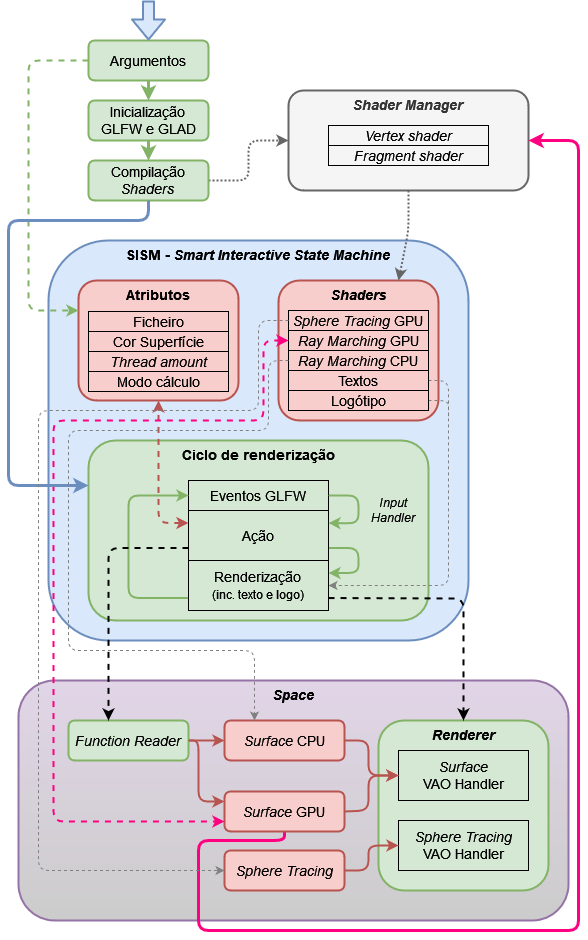
\includegraphics[width=.8\textwidth]{fluxo}
%	\caption[Fluxo de execução da \theapp]{Representação esquemática do fluxo da \theapp.}
%	\label{fig::fluxo}
%\end{figure}



\subsection{Parâmetros de arranque}
\label{ssec::impl:estrutura:start}

O programa disponibiliza uma coleção de argumentos que podem ser passados pela linha de comandos (ou terminal) para alterar o seu comportamento:

\begin{itemize}
    \item \verb|--width| ou \verb|-W|:\\
    Modifica a largura da janela de renderização, em pixeis.\\
    \textit{Default}: 600.\\
    Exemplo: \verb|-W 1000| inicia o programa com uma largura de 1000 pixeis.
    
    \item \verb|--height| ou \verb|-H|:\\
    Modifica a altura da janela de renderização, em pixeis.\\
    \textit{Default}: 600.\\
    Exemplo: \verb|-H 1000| inicia o programa com uma altura de 1000 pixeis.

    \item \verb|--render| ou \verb|-r|:\\
    Define qual o motor de renderização a que o programa recorre.\\
    Existem três modos implementados:
    \begin{itemize}[nosep]
        \item \verb|CPU|: motor de renderização por \textit{software} com uso do algoritmo naïve \textit{ray marching};
        \item \verb|GPU|: motor de renderização por aceleração de \textit{hardware} com uso do algoritmo naïve \textit{ray marching};
        \item \verb|SPHERES|: permite ao motor de renderização usar uma demonstração do algoritmo \textit{sphere tracing};
    \end{itemize}
	\textit{Default}: \verb|GPU|.
    
    \item \verb|--threads| ou \verb|-t|:\\
    Indica o número de \textit{threads} que devem ser usadas pelo motor de renderização por \textit{software}.\\
    \textit{Default}: metade do número de núcleos lógicos disponibilizados pela \ac{CPU}.\\
    Só é considerada caso o modo de renderização seja \verb|CPU|. Se o número especificado for superior ao \textit{default}, o utilizador é alertado para a possibilidade de problemas de \textit{performance} no seu sistema.\\
    Exemplo: \verb|-t 6| inicia o programa com seis \textit{threads} prontas a serem usadas.
\end{itemize}

Está ainda disponível o comando de ajuda descrito como o argumento \verb|--help| ou \verb|-h|, nesta situação o programa emite a informação descrevendo os argumentos disponíveis e em seguida este sai do programa.

O processamento destes argumentos define o estado dos seguintes atributos da \ac{SISM}:
\begin{itemize}[nosep]
    \item Motor de renderização;
    \item Resolução da janela.
\end{itemize}


\subsection{\textit{Shader Manager}}
\label{ssec::impl:estrutura:shaders}

Este passo de arranque do programa só é feito caso a inicialização das bibliotecas/\textit{frameworks} GLFW e \ac{GLAD} seja corretamente efetuada.

Os \textit{shaders} são carregados pelo \textit{Shader Manager}, o qual é instanciado para cada um dos cinco programas (num total de dez \textit{shaders} a compilar, cada um com o seu respetivo \textit{vertex} e \textit{fragment shaders}):

\begin{enumerate}[nosep]
	\item Motor de renderização por \acs{CPU};
	\item Motor de renderização acelerado por \textit{hardware} (\acs{GPU});
	\item Motor de teste de \textit{sphere tracing} (por \acs{GPU});
	\item Logótipo;
	\item Textos.
\end{enumerate}

Anteriormente à compilação dos mesmos é efetuada uma \textbf{verificação automática} dos \textit{shaders}. Caso algum esteja em falta, o programa é capaz de criar o respetivo \textit{shader} predefinido e procede à sua compilação.

Assim que todos os \textit{shaders} sejam corretamente compilados, é gerada uma janela com a dimensão definida pelo atributo do \ac{SISM}. É esperado em caso de sucesso o seguinte \textit{output}:

\begin{verbatim}
Lauching CalcGL...
    Setting global variables...     
    Setting relevant directories... [OK]
    Initializing GLFW and GLAD... [OK]
    Auto-checking shaders... (corrected 0 shaders) [OK]
    Loading shaders... [OK]
    Loading text renderer... [OK]
    Loading logo... [OK]
Done.
\end{verbatim}


\section{Motores de renderização}
\label{sec::impl:motor}

Dos três modos de renderização disponibilizados, dois são motores propriamente ditos (por \textit{software} e acelerado por \textit{hardware}) e o terceiro é um modo de demonstração de \textit{sphere tracing}. Nos dois primeiros, as funções são obtidas por ficheiros externos com a extensão \verb|*.function|. É obrigatório que as funções estejam escritas segundo a sintaxe da linguagem \ac{GLSL}.


\subsection{Cálculo por \textit{Software}}
\label{ssec::impl:motor:cpu}

Este motor de renderização pode executar em várias \textit{threads}, onde cada uma processa um conjunto de linhas contíguas do plano de visualização. As funções são processadas pela biblioteca \textit{CParse} e o algoritmo de \textit{ray marching} utilizado é o \textbf{naïve com \textit{bisection}}.


\subsection{Aceleração por \textit{hardware}}
\label{ssec::impl:motor:gpu}

O motor de renderização acelerado por \textit{hardware} faz a \textbf{injeção de funções} no \textit{fragment shader} utilizado por este modo. Uma vez que o \textit{Shader Manager} pode compilar programas a qualquer momento, as funções lidas do ficheiro \verb|*.function| são injetadas num local predeterminado do \textit{fragment shader} padrão e um novo programa é compilado com este novo \textit{shader}, sendo o anterior descartado.

A parte do \textit{fragment shader} modificado é o seguinte:

\begin{minted}[linenos]{glsl}
// Defines a implicit function
float evalImplicitFunc(vec3 point) {
    float x = point.x;
    float y = point.y;
    float z = point.z;
    float prod = 1.f;

    // <gamma conditions>

    return prod;
}
\end{minted}

As funções lidas são multiplicadas a fim de formar uma Superfície $\Pi$ com um fator de \textit{blending} $r = 0$. A sua injeção é feita no local do comentário indicado por \verb|<gamma conditions>|. Por exemplo, caso o ficheiro defina três esferas:

\begin{eqnarray*}
	x^2 + y^2 + z^2 - 1 = 0 \\
	(x-2)^2 + (y-1)^2 + z^2 - 1 = 0 \\
	(x-1)^2 + (y-2)^2 + (z-2)^2 - 1 = 0
\end{eqnarray*}

O \textit{fragment shader} será recompilado com as seguintes linhas de código no lugar de \verb|<gamma conditions>|.

\begin{minted}[linenos,firstnumber=8]{glsl}
prod *= pow(x, 2.) + pow(y, 2.) + pow(z, 2.) - 1.;
prod *= pow(x-2., 2.) + pow(y-1., 2.) + pow(z, 2.) - 1.;
prod *= pow(x-1., 2.) + pow(y-2., 2.) + pow(z-2., 2.) - 1.;
\end{minted}

Este modo \textbf{não implementa \textit{bisection}} devido a uma limitação ao nível da \acs{GPU}.

Sendo unidades de cálculo muito especializadas, as \acsp{GPU} não contemplam instruções de \textit{interrupt}, cuja consequência é a impossibilidade de parar os programas por si executados (conjunto de \textit{shaders}) uma vez iniciados. Os \textit{shaders} podem entrar em ciclos infinitos, os quais levariam ao total bloqueio de todo o sistema operativo por indisponibilidade da \acs{GPU}. Desta forma, o sistema operativo monitoriza o tempo de cada execução da \acs{GPU} e, caso ultrapasse um determinado \textit{threshold} por si definido, é-lhe feito um \textit{reset}.

Por este motivo, a implementação de \textit{bisection} levou a este fenómeno de \textit{reset} da \acs{GPU}, pelo que foi excluído do algoritmo final implementado no \textit{fragment shader}.

Há ainda a notar que este motor não verifica as funções fornecidas nos ficheiros \verb|*.function| uma vez que não se enquadrava no objetivo principal do projeto.


\subsection{Demonstração de \textit{Sphere Tracing}}
\label{ssec::impl:motor:sphere}

O modo de demonstração de \textit{sphere tracing} distingue-se dos demais uma vez que implementa diretamente no seu \textit{fragment shader} as superfícies a serem renderizadas, estando então as respetivas \acfp{SDF} presentes diretamente no código. Outras funções implícitas não podem ser renderizadas, servindo então para mero efeito ilustrativo deste algoritmo de \textit{ray marching}.


%\section{Conclusões}
%\label{sec::impl:conc}

	\clearpage{\thispagestyle{empty}\cleardoublepage}
	\chapter{Testes e Resultados}
\label{ch::testes}

%\section{Introdução}
%\label{sec::testes:intro}

Durante a implementação e após a conclusão da versão final do projeto \theapp, foram realizados diversos testes a fim de analisar a exatidão do algoritmo e a qualidade das renderizações obtidas.

Doravante, referir-se-á ao programa final exclusivamente pelo seu nome, \theapp.


\section{Arranque e \textit{Setup} Inicial}
\label{sec::testes::start}

A \theapp~permite modular o seu comportamento através de argumentos passados por linha de comandos. Este é o passo de \textit{setup} inicial do programa.

\begin{itemize}
	\item \verb|-r| (\textit{render mode}): permite definir qual o motor de renderização a ser usado. As opções são:
	\begin{itemize}[nosep]
		\item \verb|CPU|: motor de renderização por \textit{software} (faz usufruto da \ac{CPU});
		\item \verb|GPU|: aceleração por \textit{hardware} (com recurso à \ac{GPU}).
	\end{itemize}
	
	\item \verb|-t| (\textit{threads}): permite definir o número de \textit{threads} a serem usadas no motor de renderização por \textit{software}. Por defeito irá utilizar metade dos núcleos lógicos disponíveis. Caso o utilizador defina um número superior, um aviso é emitido sobre a potencial perda de \textit{performance}.
\end{itemize}

O programa irá carregar todos os recursos necessários ao seu bom funcionamento, em particular:
\begin{itemize}[nosep]
	\item Bibliotecas e \textit{frameworks} (GLFW e \acs{GLAD});
	\item \textit{Shaders} para texto, logótipo e superfície implícita;
	\item Fonte para o texto e imagem do logótipo;
\end{itemize}

Em caso de erro, o programa não arranca e a sua execução é abortada. Em caso de sucesso, é apresentada uma janela com a \textit{home screen} do programa (Figura \ref{fig::home}). O utilizador pode selecionar o ficheiro com as funções a renderizar pressionando a tecla \verb|O|.


\section{Testes em Fase de Desenvolvimento}
\label{sec::teste:dev}

A fase de desenvolvimento englobou duas fases distintas:
\begin{enumerate}[nosep]
	\item Declaração das funções implícitas em código \acs{GLSL} de forma direta no \textit{fragment shader};
	\item Injeção das funções implícitas lidas a partir de ficheiros externos.
\end{enumerate}



\begin{figure}[!htbp]
	\centering
	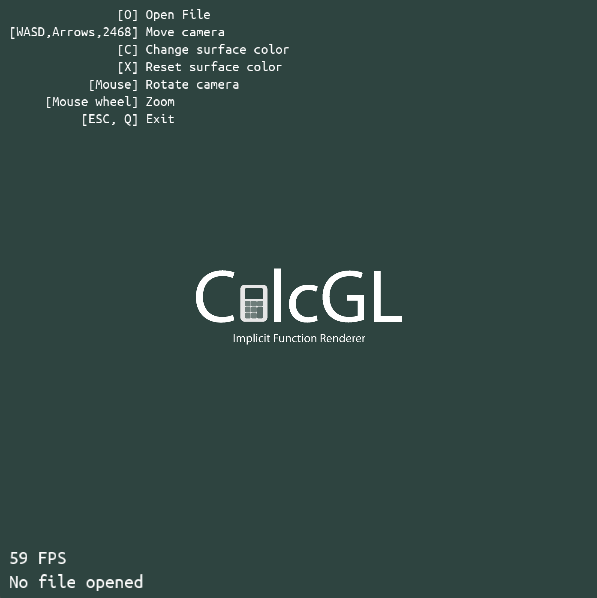
\includegraphics[width=.8\textwidth]{home}
	\caption[Ecrã inicial da aplicação]{Ecrã inicial da aplicação \theapp.}
	\label{fig::home}
\end{figure}

\begin{figure}[!htbp]
	\centering
	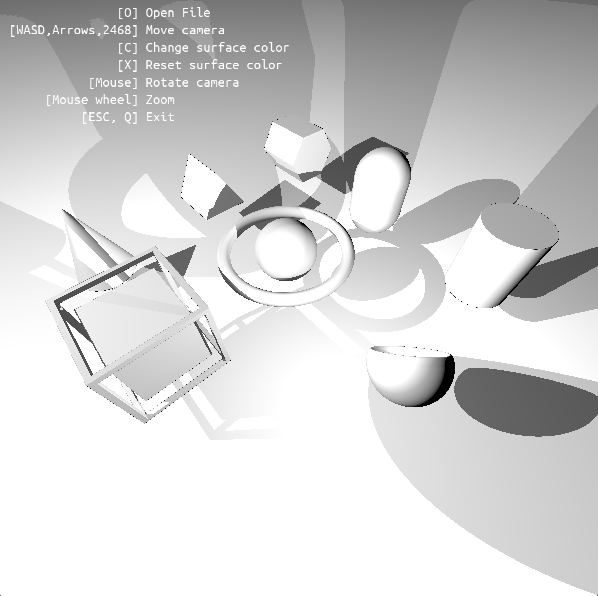
\includegraphics[width=.8\textwidth]{sphereoriginal}
	\caption[Nove objetos com \textit{sphere tracing} no \theapp]{Renderização de nove objetos no \theapp~usando o algoritmo de \textit{sphere tracing}.}
	\label{fig::sphereoriginal}
\end{figure}

\begin{figure}[!htbp]
	\centering
	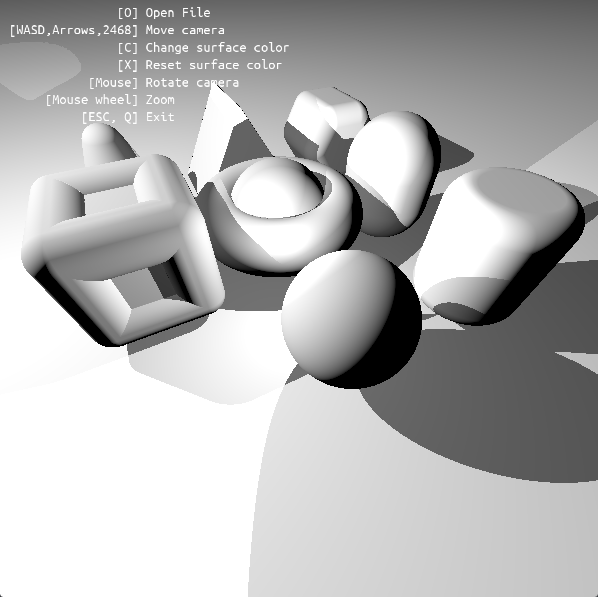
\includegraphics[width=.8\textwidth]{spheresmooth}
	\caption[Nove objetos com \textit{sphere tracing} e suavização no \theapp]{Renderização de nove objetos no \theapp~usando o algoritmo de \textit{sphere tracing} com um fator de suavização $s$ dependente do tempo de execução $t$, em particular $s = \cos(t)$.}
	\label{fig::spheresmooth}
\end{figure}

\begin{figure}[!htbp]
	\centering
	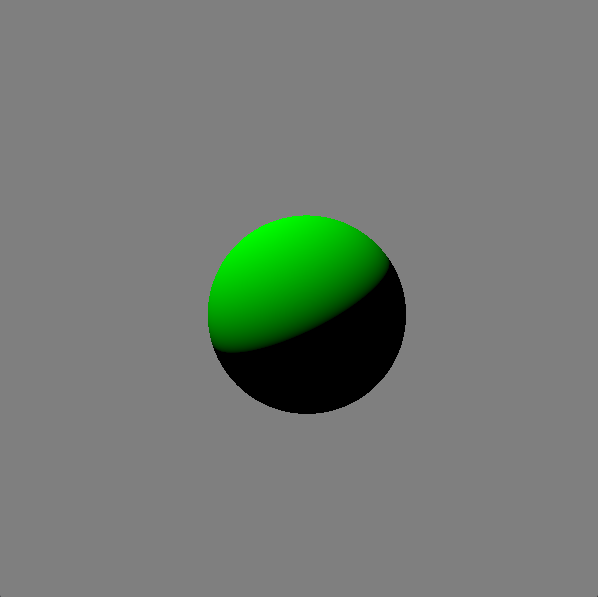
\includegraphics[width=.8\textwidth]{calcglsphere}
	\caption[Esfera no \theapp~com algoritmo naïve]{Esfera renderizada no \theapp, em fase inicial de testes, com o algoritmo naïve.}
	\label{fig::calcglsphere}
\end{figure}

\begin{figure}[!htbp]
	\centering
	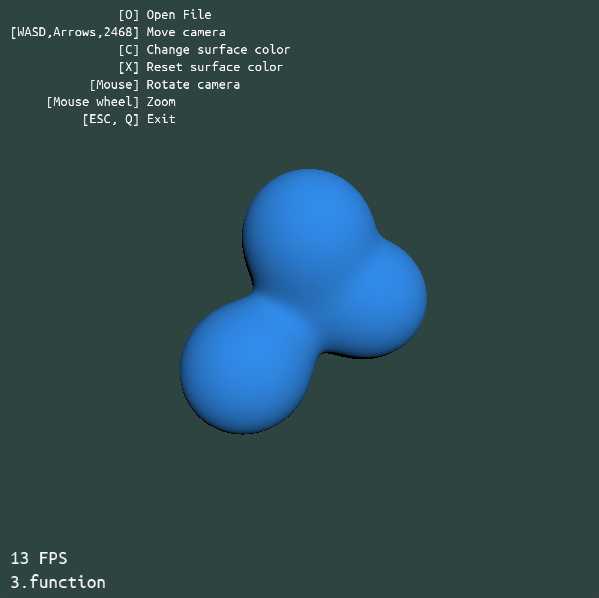
\includegraphics[width=.8\textwidth]{calcglpisurf}
	\caption[Superfície $\Pi$ no \theapp~com algoritmo naïve]{Superfície $\Pi$ renderizada no \theapp~com algoritmo naïve.}
	\label{fig::calcglpisurf}
\end{figure}

\begin{figure}[!htbp]
	\centering
	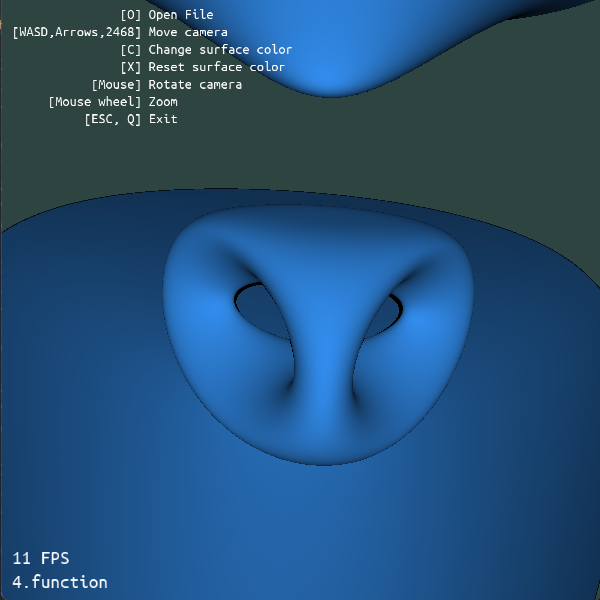
\includegraphics[width=.8\textwidth]{calcglgenus}
	\caption[\textit{Genus} no \theapp~com algoritmo naïve]{\textit{Genus} renderizado no \theapp~com algoritmo naïve.}
	\label{fig::calcglgenus}
\end{figure}




\begin{table}[!htbp]
	\centering
	\caption[Tempos de renderização em \acs{CPU}]{Tempo para a renderização de uma única \textit{frame} com recurso à \acs{CPU} para diferentes números de \textit{threads}. Os testes foram realizados no computador \textit{desktop} listado na Tabela \ref{tab::hardware}.}
	\label{tab::render_cpu}
	\begin{tabular}{r r r}
		\toprule
		\multirow{2}{*}{\textbf{Threads}} & \multicolumn{2}{c}{\textbf{Tempo}} \\
		\cline{2-3}
		& Segundos & h:m's'' \\
		\midrule
		1 &  7087 & 01:58'07'' \\
		2 &  5984 & 01:39'44'' \\
		4 &  7566 & 02:06'06'' \\
		6 & 10414 & 02:53'34'' \\
		\bottomrule
	\end{tabular}
\end{table}


%\section{Conclusões}
%\label{sec::testes:conc}

	\clearpage{\thispagestyle{empty}\cleardoublepage}
	\chapter{Conclusões e Trabalho Futuro}
\label{ch::conc}

\section{Conclusões}
\label{sec::conc:conc}

\todo{}


\section{Trabalho Futuro}
\label{sec::conc:futuro}

\todo{}

	\clearpage{\thispagestyle{empty}\cleardoublepage}
	
	% SE EXISTIREM APENDICES, DESCOMENTAR O QUE ESTÁ EM BAIXO
	% \appendix
	% \include{apendice1}
	% \clearpage{\pagestyle{empty}\cleardoublepage}
	% \include{continuacao}
	% \clearpage{\pagestyle{empty}\cleardoublepage}
	% \include{apendice2}
	% \clearpage{\pagestyle{empty}\cleardoublepage}
	% \include{apendice3}
	% \clearpage{\pagestyle{empty}\cleardoublepage}
	
	\backmatter
	
	\bibliographystyle{IEEEtran}
	\bibliography{bibliografia.bib}
\end{document}